\documentclass[border=8pt]{standalone}
\usepackage{tikz}
\usetikzlibrary{arrows.meta,positioning,calc}
\begin{document}
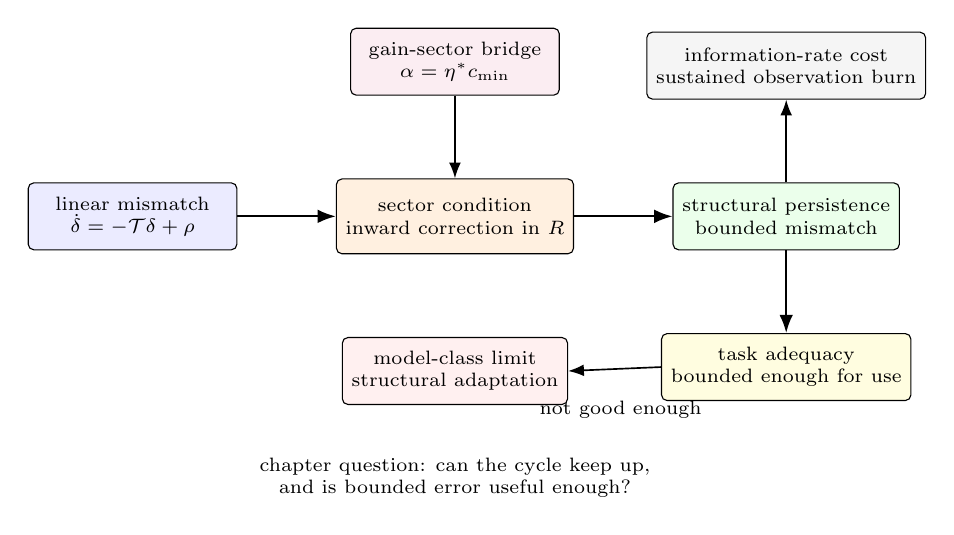
\begin{tikzpicture}[
  box/.style={draw, rounded corners=2pt, align=center, minimum width=2.65cm, minimum height=0.85cm, font=\scriptsize},
  key/.style={draw, rounded corners=2pt, align=center, minimum width=3.0cm, minimum height=0.95cm, font=\scriptsize, fill=orange!12},
  note/.style={align=center, font=\scriptsize},
  arr/.style={-Latex, thick},
  thinarr/.style={-Latex, semithick}
]

\node[box, fill=blue!8] (ode) {linear mismatch\\$\dot\delta=-\mathcal T\delta+\rho$};
\node[key, right=1.25cm of ode] (sector) {sector condition\\inward correction in $R$};
\node[box, fill=green!8, right=1.25cm of sector] (persist) {structural persistence\\bounded mismatch};
\draw[arr] (ode) -- (sector);
\draw[arr] (sector) -- (persist);

\node[box, fill=yellow!12, below=1.05cm of persist] (task) {task adequacy\\bounded enough for use};
\draw[arr] (persist) -- (task);

\node[box, fill=red!6, below=1.05cm of sector] (struct) {model-class limit\\structural adaptation};
\draw[thinarr] (task.west) -- (struct.east);
\node[note, below=0.28cm of $(task)!0.5!(struct)$] {not good enough};

\node[box, fill=purple!7, above=1.05cm of sector] (gain) {gain-sector bridge\\$\alpha=\eta^\ast c_{\min}$};
\draw[thinarr] (gain) -- (sector);

\node[box, fill=gray!8, above=1.05cm of persist] (cost) {information-rate cost\\sustained observation burn};
\draw[thinarr] (persist) -- (cost);

\node[note, below=0.55cm of struct] {chapter question: can the cycle keep up,\\and is bounded error useful enough?};

\end{tikzpicture}
\end{document}
